\subsection{Inclusive Selection: Semileptonic channel}
\label{subsec:sel_incl_semilept}

Events for the semileptonic channel are obtained with HLT\_Ele27\_eta2p1\_WP75\_Gsf in MC and HLT\_Ele27\_eta2p1\_WPLoose\_Gsf in data, a single electron trigger, and HLT\_IsoMu27, a single muon trigger. Kinematic thresholds on the trigger objects constrain the offline requirements on the electron or muon to $\pt>30\:\GeV$ and $|\eta|<2.1$ in order to avoid the sharp efficiency turn-on. Trigger efficiencies measured with the tag-and-probe method are shown in Fig.~\ref{fig:seleff} and Fig.~\ref{fig:smueff} for the single electron HLT\_Ele27\_eta2p1\_WP75\_Gsf trigger measured in MC and HLT\_Ele27\_eta2p1\_WPLoose\_Gsf in data and HLT\_IsoMu27 in data and MC, respectively.

The data-to-MC trigger efficiency scale factors for the single electron HLT\_Ele27\_eta2p1\_WP75\_Gsf trigger and the single muon HLT\_IsoMu27 trigger have been computed in $\pt$-$|\eta|$ bins using standard tag-and-probe procedures and are shown in Table~\ref{tab:sf_ele} and Table~\ref{tab:sf_mu} respectively. 

\begin{table}[!ht]
\centering
\begin{tabular}{|c|c|c|c|c|}
\hline
&                                &                                &                                &                                                                 \\   
& $0.0 < |\eta| < 0.4$ & $0.4 < |\eta| < 1.4$ & $1.4 < |\eta| < 1.6$ & $1.6 < |\eta| < 2.1$    \\
&                                &                                &                                &                                                                \\   
\hline
$30 < \pt <  32$ &  $0.936 \pm  0.006$  &  $0.947 \pm  0.006$  &  $0.794 \pm  0.026$  &  $0.893 \pm  0.008$ \\
\hline
$32 < \pt <  35$ &  $0.958 \pm  0.003$  &  $0.980 \pm  0.003$  &  $0.914 \pm  0.013$  &  $0.954 \pm  0.005$ \\
\hline
$35 <\pt  <  40$ &  $0.970 \pm  0.002$  &  $0.998 \pm  0.001$  &  $0.999 \pm  0.006$  &  $0.958 \pm  0.003$ \\
\hline
$40 < \pt <  50$ &  $0.980 \pm  0.001$  &  $1.005 \pm  0.001$  &  $0.998 \pm  0.004$  &  $0.958 \pm  0.002$ \\
\hline
$50 < \pt < 200$ & $0.998 \pm  0.001$  &  $1.012 \pm  0.001$  &  $1.004 \pm  0.005$  &  $0.944 \pm  0.003$ \\
\hline
      $\pt > 200$   & $1.011 \pm  0.031$  &  $1.012 \pm  0.019$  &  $0.947 \pm  0.115$  &  $0.950 \pm  0.077 $\\	
\hline	
	
\end{tabular}
\caption{Data-to-MC efficiency scale factors for single electron trigger by $\pt$-$|\eta|$ bins}
\label{tab:sf_ele}
\end{table}


\begin{table}[!ht]
\centering
\begin{tabular}{|c|c|c|c|c|c|c|}
\hline
  &                                &                                &                                &                                 &                                &                             \\   
  & $0.0 < |\eta| < 0.4$ & $0.4 < |\eta| < 0.8$ & $0.8 < |\eta| < 1.2$ & $1.2 < |\eta| < 1.6$ & $1.6 < |\eta| < 2.1$ & $2.1 < |\eta| < 2.4$ \\
  &                                &                                &                                &                                 &                                &                             \\   

\hline
	$30 < \pt <   32$ &  $0.963 \pm  0.004$  & $ 1.004 \pm  0.003 $ &  $0.982 \pm  0.005 $ &  $0.972 \pm  0.004$  &  $0.937 \pm  0.005 $ &  $0.910 \pm  0.010$ \\
\hline	
  	$32 < \pt <   34$ &  $0.972 \pm  0.003$  & $ 1.008 \pm  0.003$  &  $0.995 \pm  0.004 $ &  $0.987 \pm  0.004 $ & $ 0.948 \pm  0.005$  & $ 0.917 \pm  0.009$ \\
\hline  	
	$34 < \pt <   36 $&  $0.979 \pm  0.003$  &  $1.003 \pm  0.002$  &  $0.988 \pm  0.004 $ &  $0.990 \pm  0.003$  &  $0.945 \pm  0.004 $ & $ 0.921 \pm  0.008 $\\
\hline  	
	$36 < \pt <   38$ &  $0.977 \pm  0.002$  &  $1.001 \pm  0.002$  &  $0.980 \pm  0.003 $ &  $0.989 \pm  0.003$  & $ 0.951 \pm  0.004 $ & $ 0.923 \pm  0.007$ \\
\hline  	
	$38 < \pt <   40$ &  $0.977 \pm  0.002$  &  $0.999 \pm  0.002$  &  $0.984 \pm  0.003$  &  $0.988 \pm  0.002$  & $ 0.955 \pm  0.003$  & $ 0.928 \pm  0.007$ \\
\hline  	
	$40 < \pt <   45$ &  $0.977 \pm  0.001$  &  $0.996 \pm  0.001$  &  $0.978 \pm  0.002$  &  $0.990 \pm  0.001$  &  $0.955 \pm  0.002 $ &  $0.934 \pm  0.004 $\\
\hline  	
	$45 < \pt <   50$ &  $0.978 \pm  0.001$  & $ 0.996 \pm  0.001$  &  $0.979 \pm  0.002$  &  $0.993 \pm  0.001$  &  $0.956 \pm  0.002 $ & $ 0.939 \pm  0.004$ \\
\hline  	

	$50 < \pt <  200$ &  $0.977 \pm  0.002$  &  $0.994 \pm  0.001$  &  $0.976 \pm  0.002$  &  $0.994 \pm  0.001$  &  $0.958 \pm  0.002$  &  $0.955 \pm  0.004$ \\

\hline      	
	 $\pt >  200$ &  $0.993 \pm  0.031$  &  $0.998 \pm  0.027$  &  $1.005 \pm  0.047$  &  $0.982 \pm  0.038$  &  $0.959 \pm  0.062 $ &  $0.822 \pm  0.114 $\\
\hline
\end{tabular}
\caption{Data-to-MC efficiency scale factors for single muon HLT\_IsoMu27 by $\pt$-$|\eta|$ bins}
\label{tab:sf_mu}
\end{table}


\begin{figure}[htbp]
  \centering
  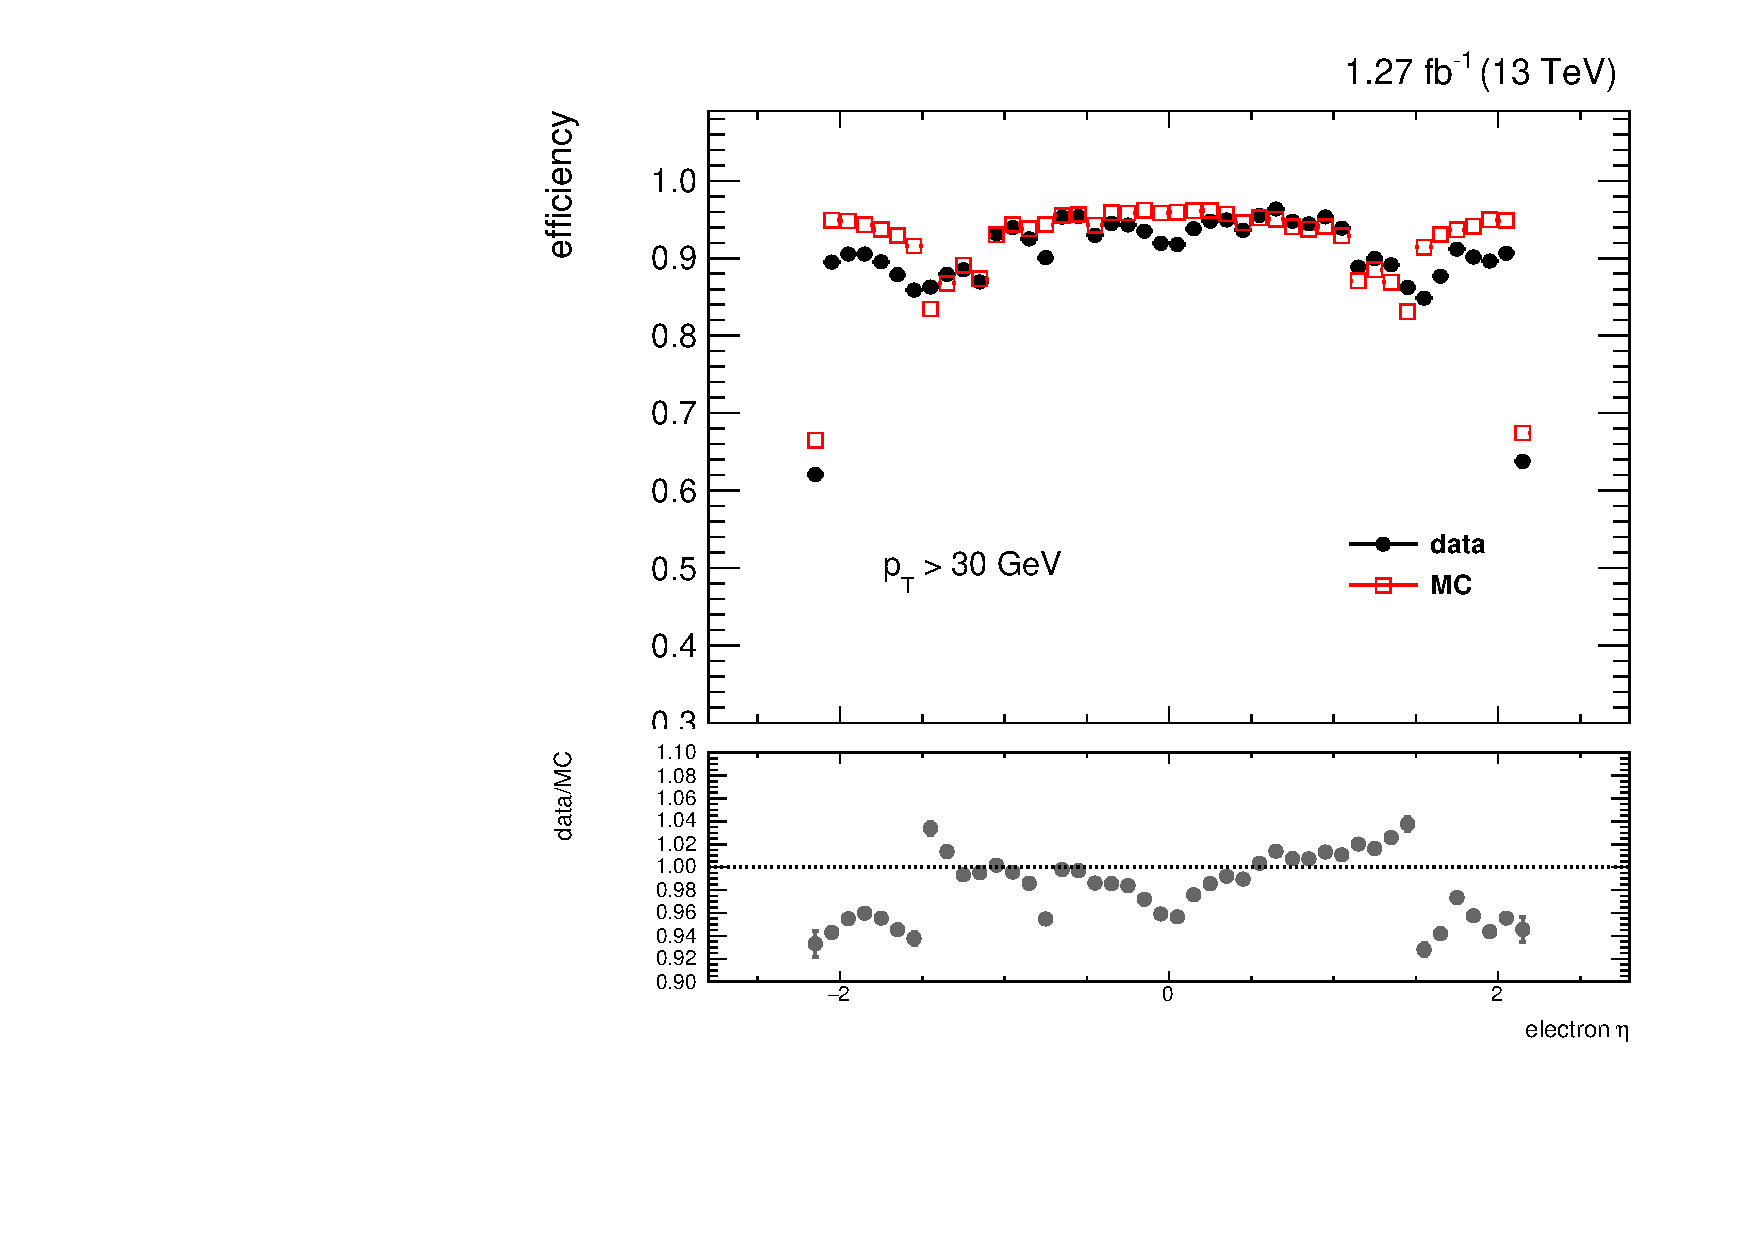
\includegraphics[width=0.48\textwidth]{figures/sel_effeta_dataMC.pdf}
  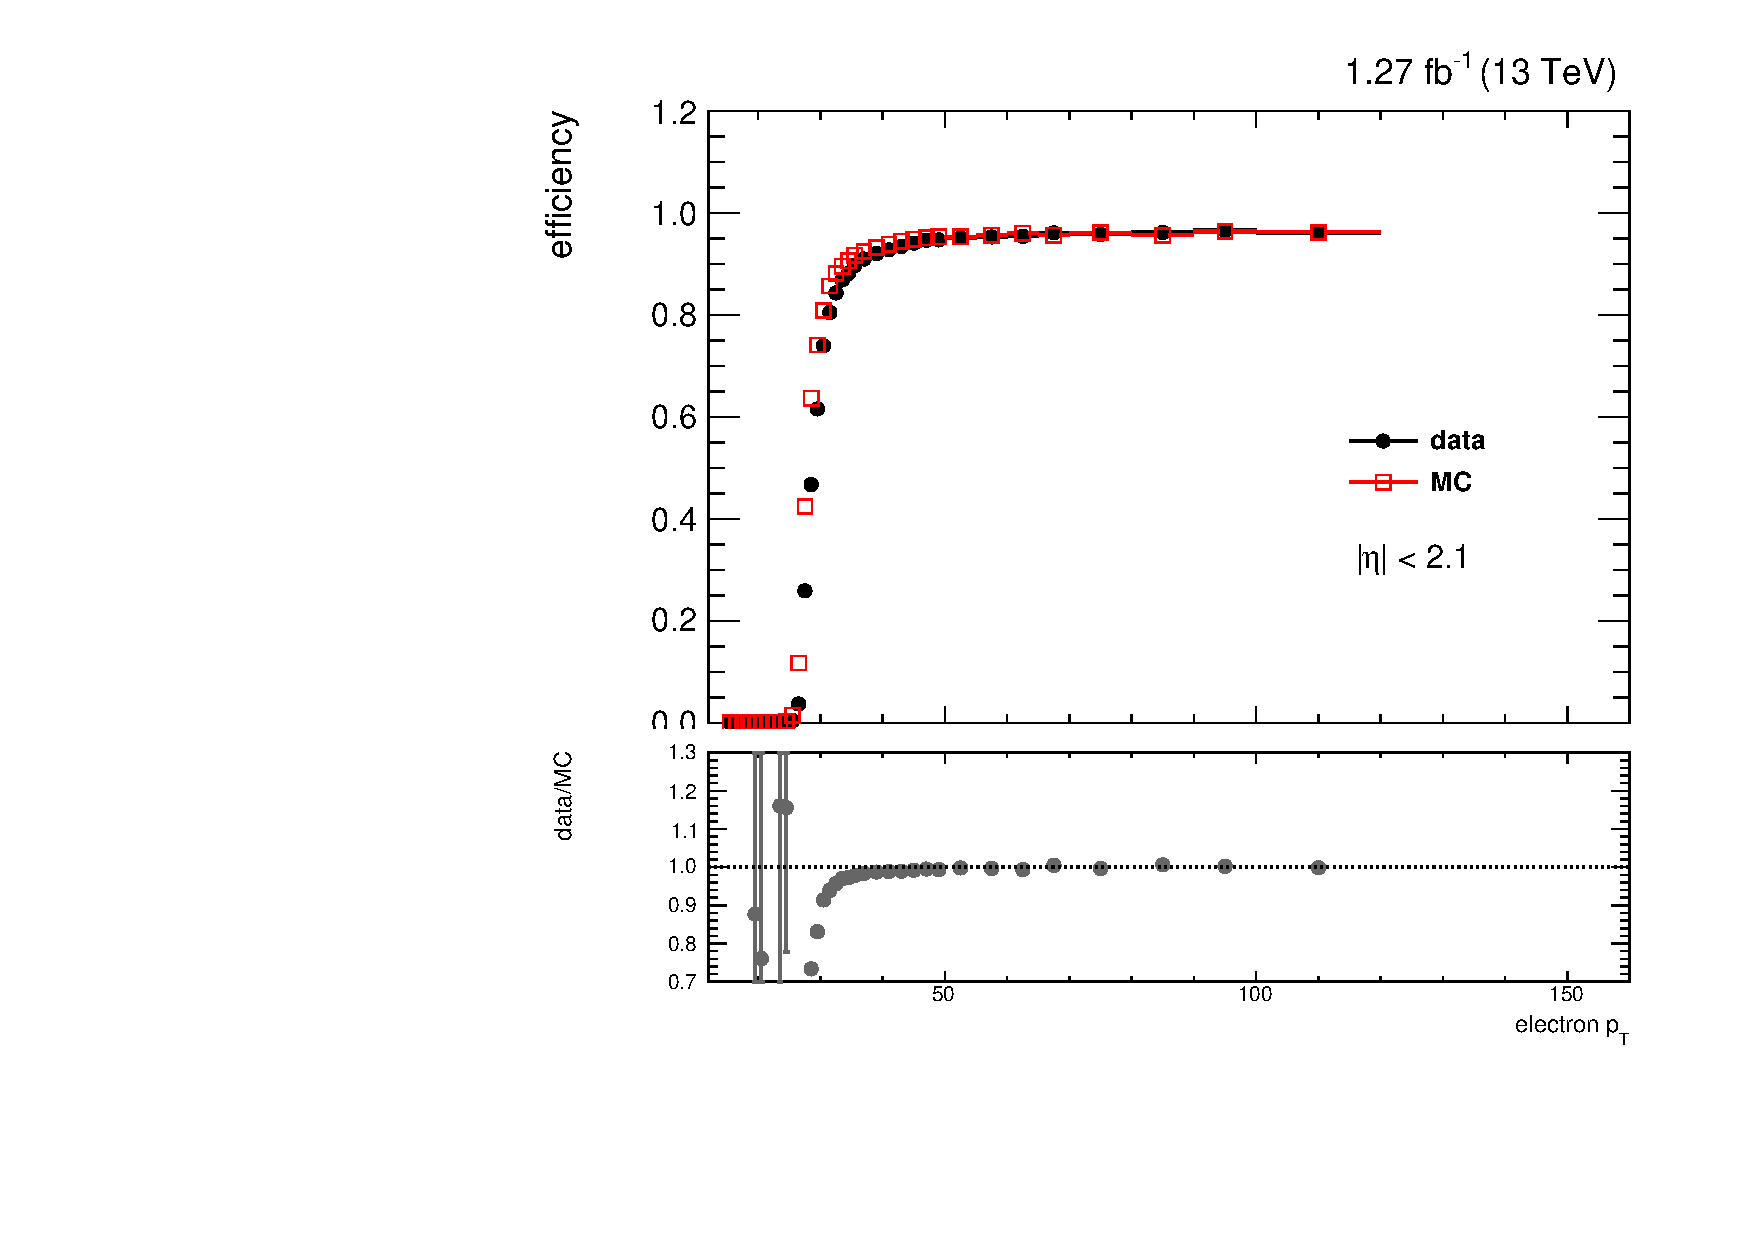
\includegraphics[width=0.48\textwidth]{figures/sel_effpt_dataMC.pdf}
  \caption{Efficiency of HLT\_Ele27\_eta2p1\_WP75\_Gsf in MC and HLT\_Ele27\_eta2p1\_WPLoose\_Gsf in data with respect to $\eta$ (left) and $\pt$ for $|\eta|<2.1$ (right).}
  \label{fig:seleff}
\end{figure}

\begin{figure}[htbp]
  \centering
  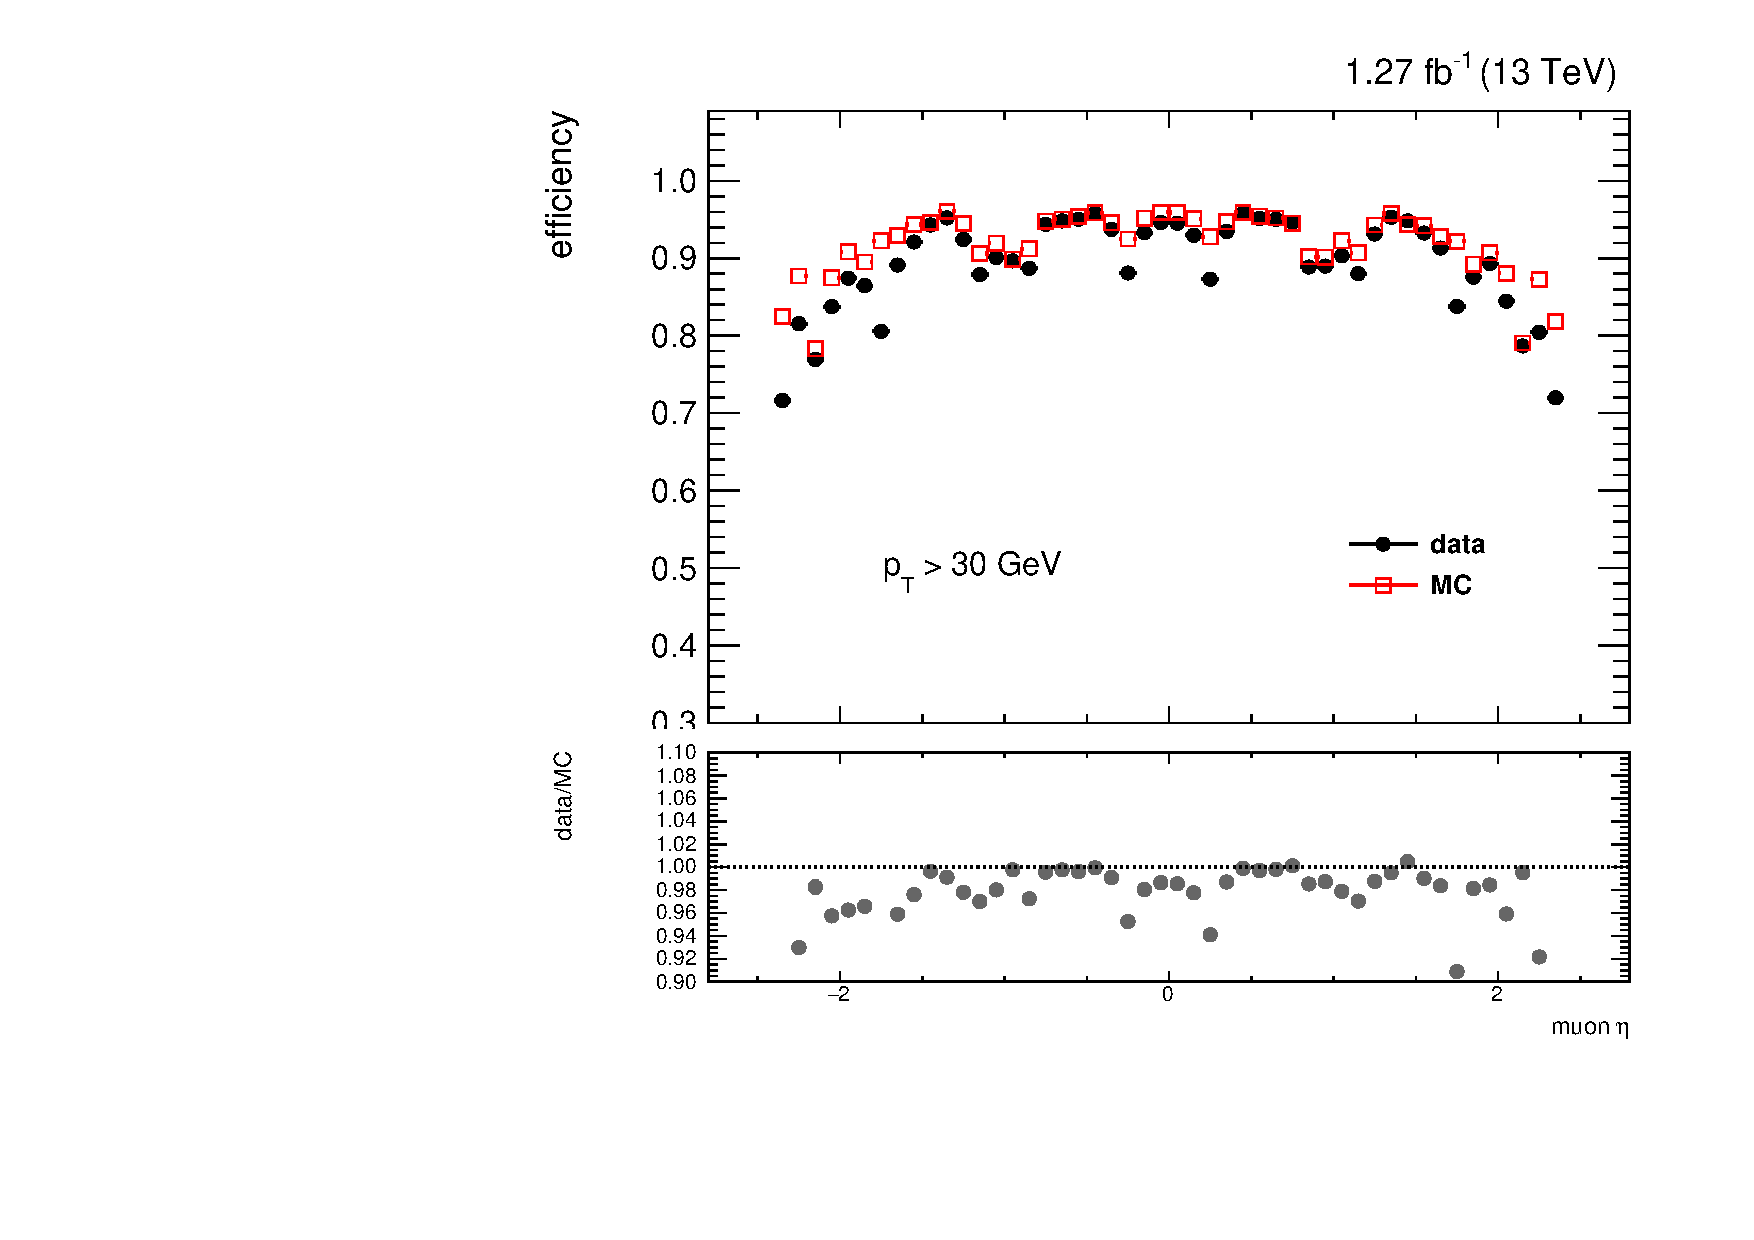
\includegraphics[width=0.48\textwidth]{figures/smu_effeta_dataMC.pdf}
  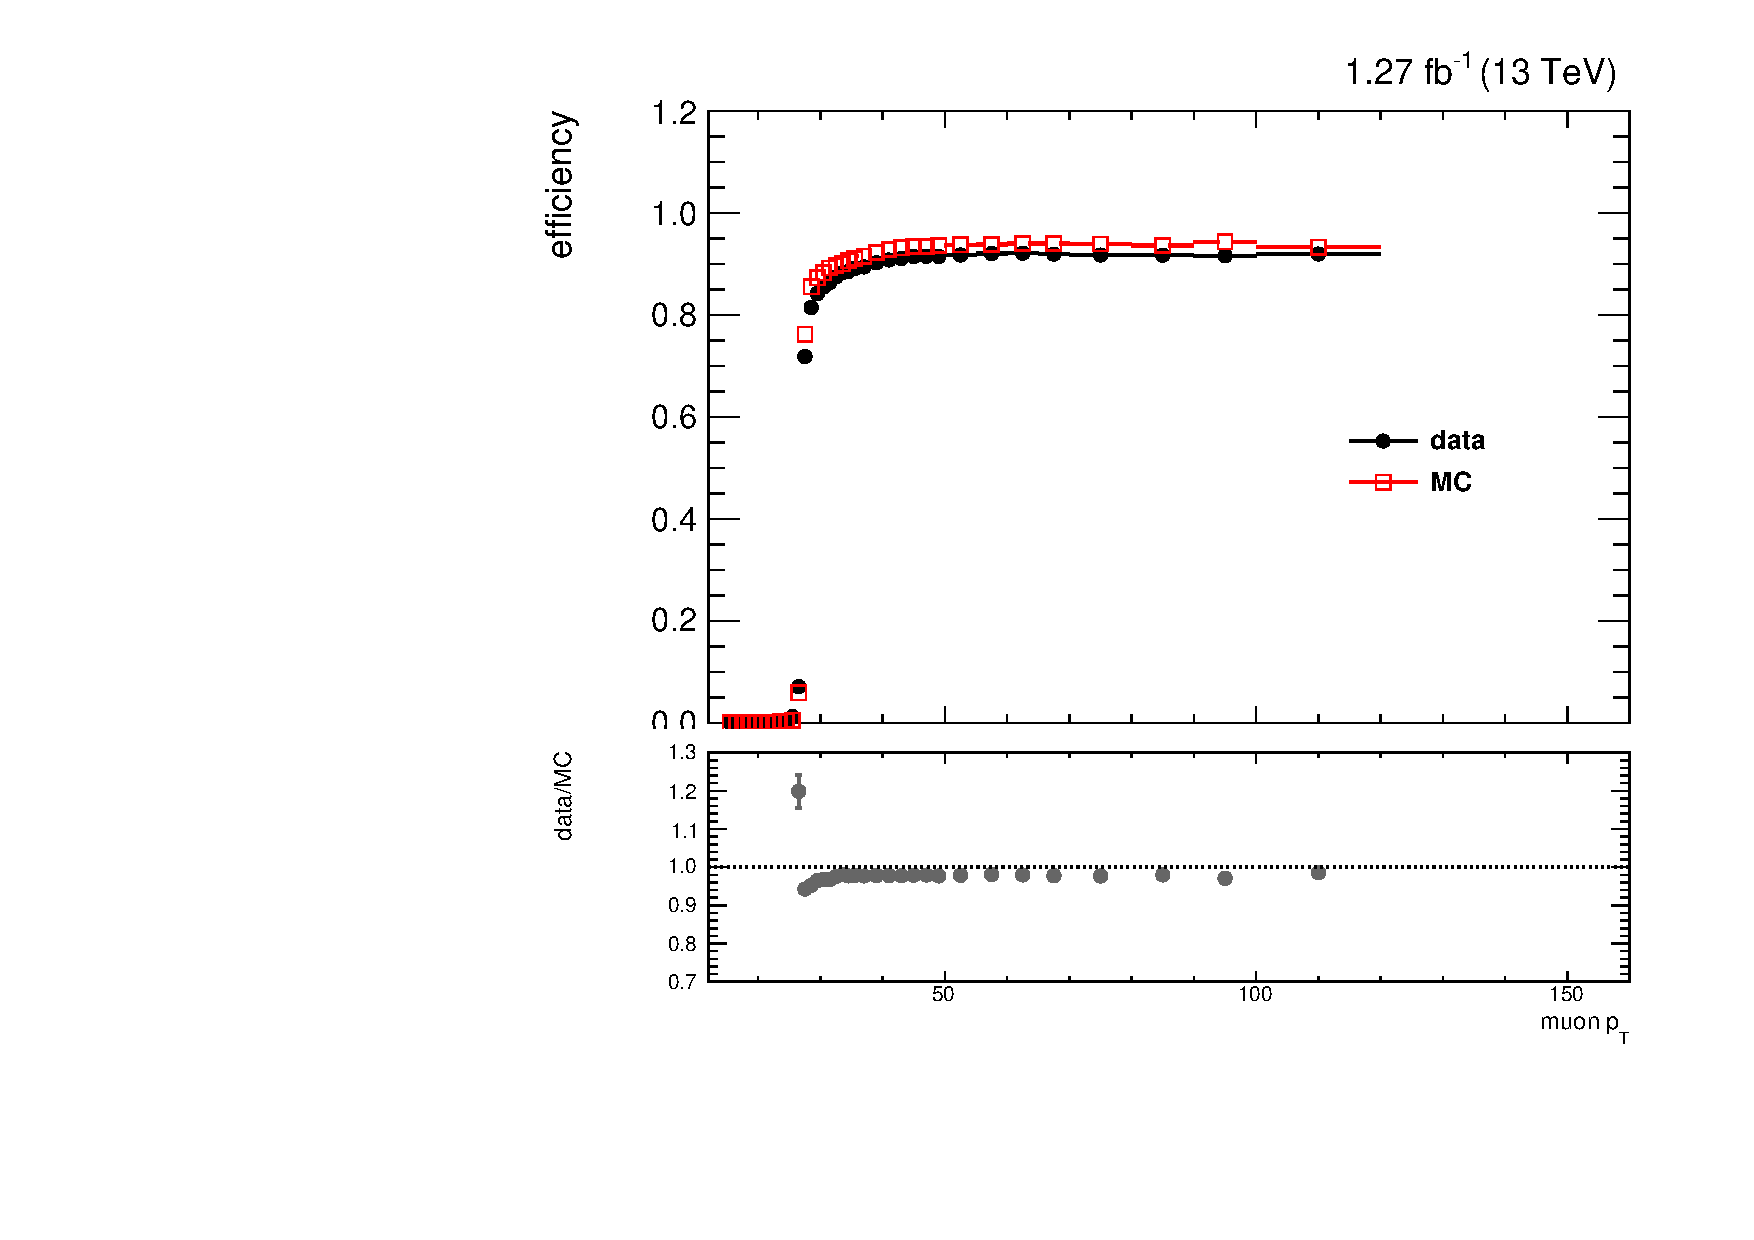
\includegraphics[width=0.48\textwidth]{figures/smu_effpt_dataMC.pdf}
  \caption{Efficiency of HLT\_IsoMu27 in data and MC with respect to $\eta$ (left) and $\pt$ for $|\eta|<2.4$ (right).}
  \label{fig:smueff}
\end{figure}

\clearpage

In order to greatly reduce semileptonic $\ttbar$ and $\Wjets$ background, events are required to have high transverse mass, $M_T$, defined as,
\begin{equation}
M_T = \sqrt{2\,\pt^{\Lep}\,\met \left(1-\cos\Delta\phi_{\Lep,\met}\right)}.
\end{equation}

The remaining $\ttbar$ background is predominantly from the dilepton channel. Two variables that help reject this background are $M_{T2}^W$ and $\min_{i=1,2}\Delta\phi\left(j_i,\met\right)$, the minimum $\Delta\phi$ between jet and $\met$ among the two leading jets. The offline event selection is,
\begin{itemize}
\item $\met > 160\:\GeV$,
\item exactly one electron or muon passing ``Tight'' selection with $\pt>30\:\GeV$ and $|\eta|<2.1$ and matched to the trigger object,
\item at least $3$ AK4CHS jets with $\pt>30\:\GeV$ and $|\eta|<4$,
  \begin{itemize}
  \item at least one of which has $|\eta|<2.4$ and $\Bot$-tagged,
  \end{itemize}
\item no additional muons passing ``Loose'' selection with $\pt>10\:\GeV$ and $|\eta|<2.4$,
\item no additional electrons passing ``Veto'' selection with $\pt>10\:\GeV$ and $|\eta|<2.5$,
\item $M_T > 160\:\GeV$,
\item $M_{T2}^W > 200\:\GeV$,
\item $\min_{i=1,2}\Delta\phi\left(j_i,\met\right)>1.2$.
\end{itemize}

\begin{figure}[htbp]
  \centering
  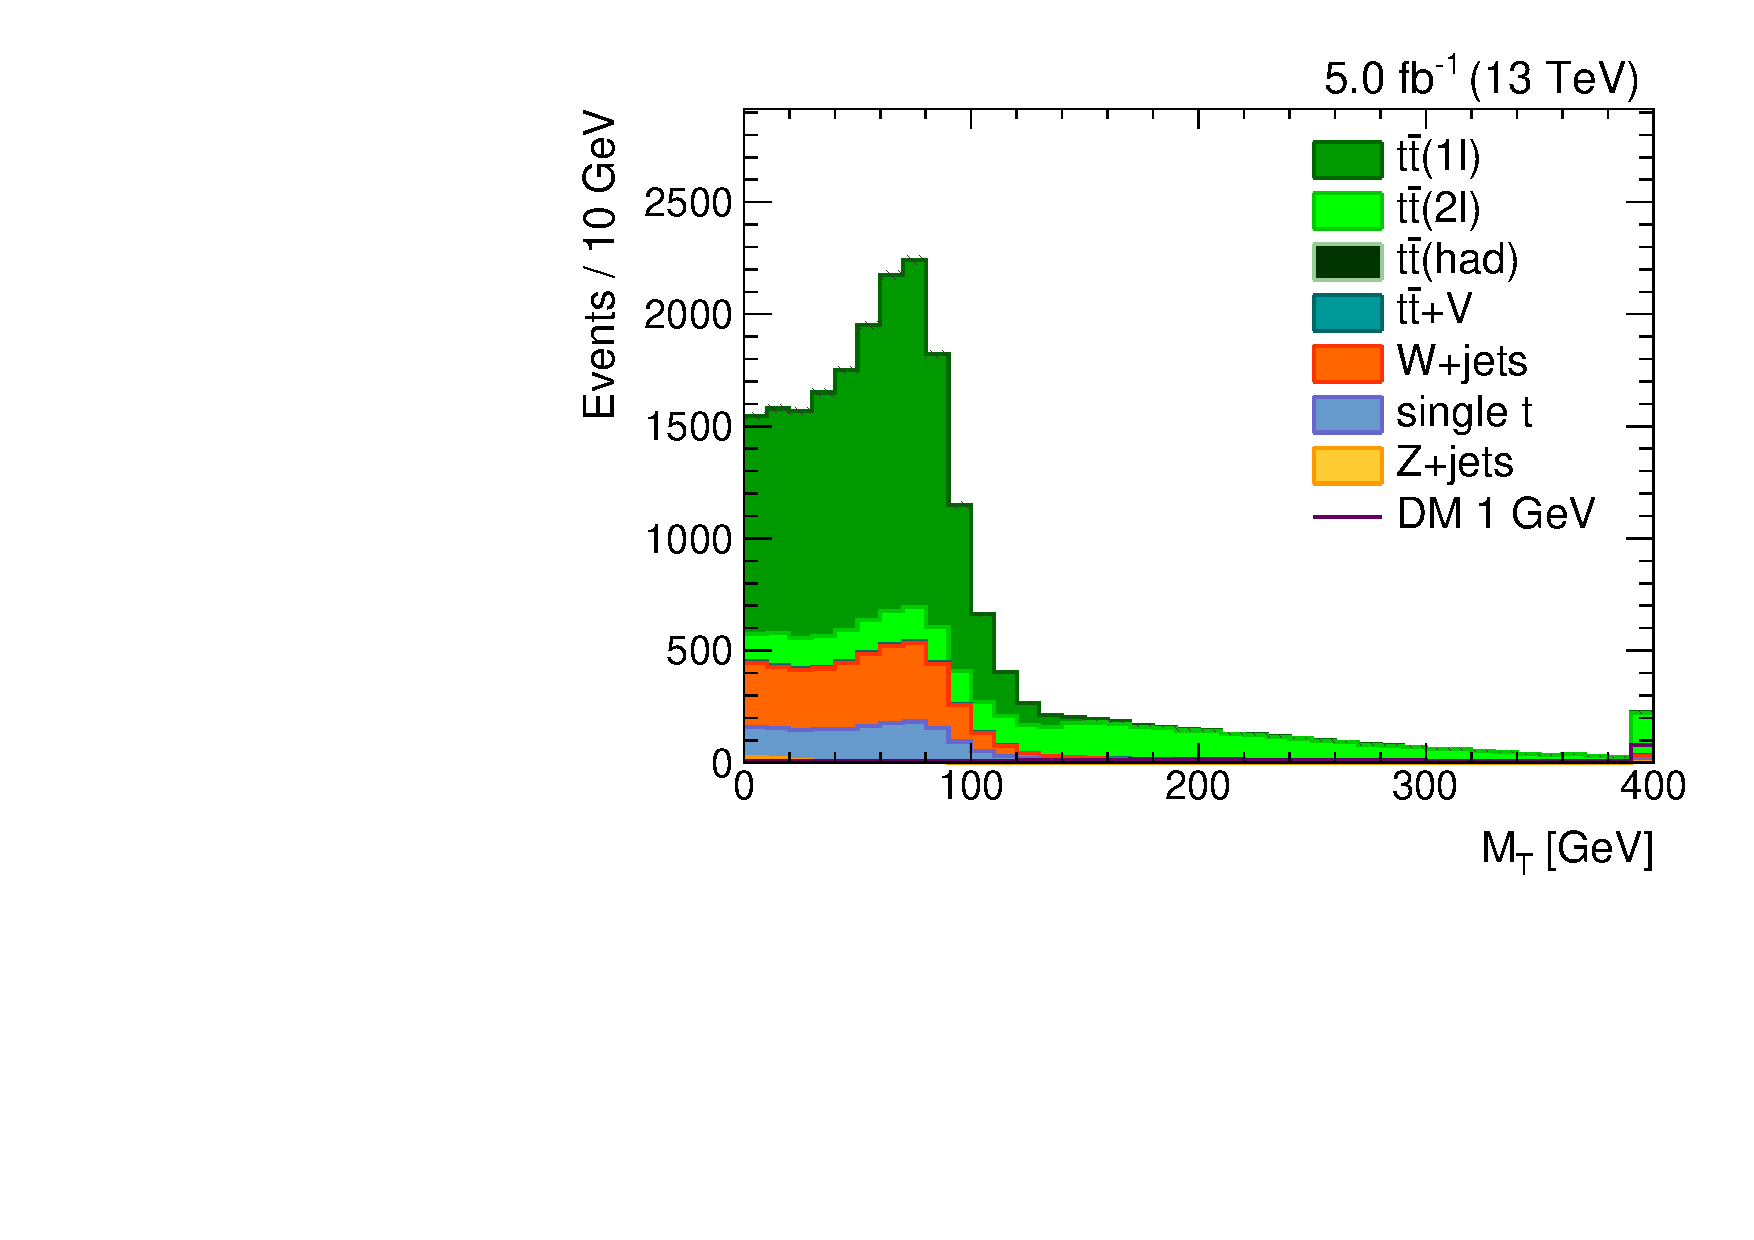
\includegraphics[width=0.48\textwidth]{figures/semilept-incl-mt_l.pdf}
  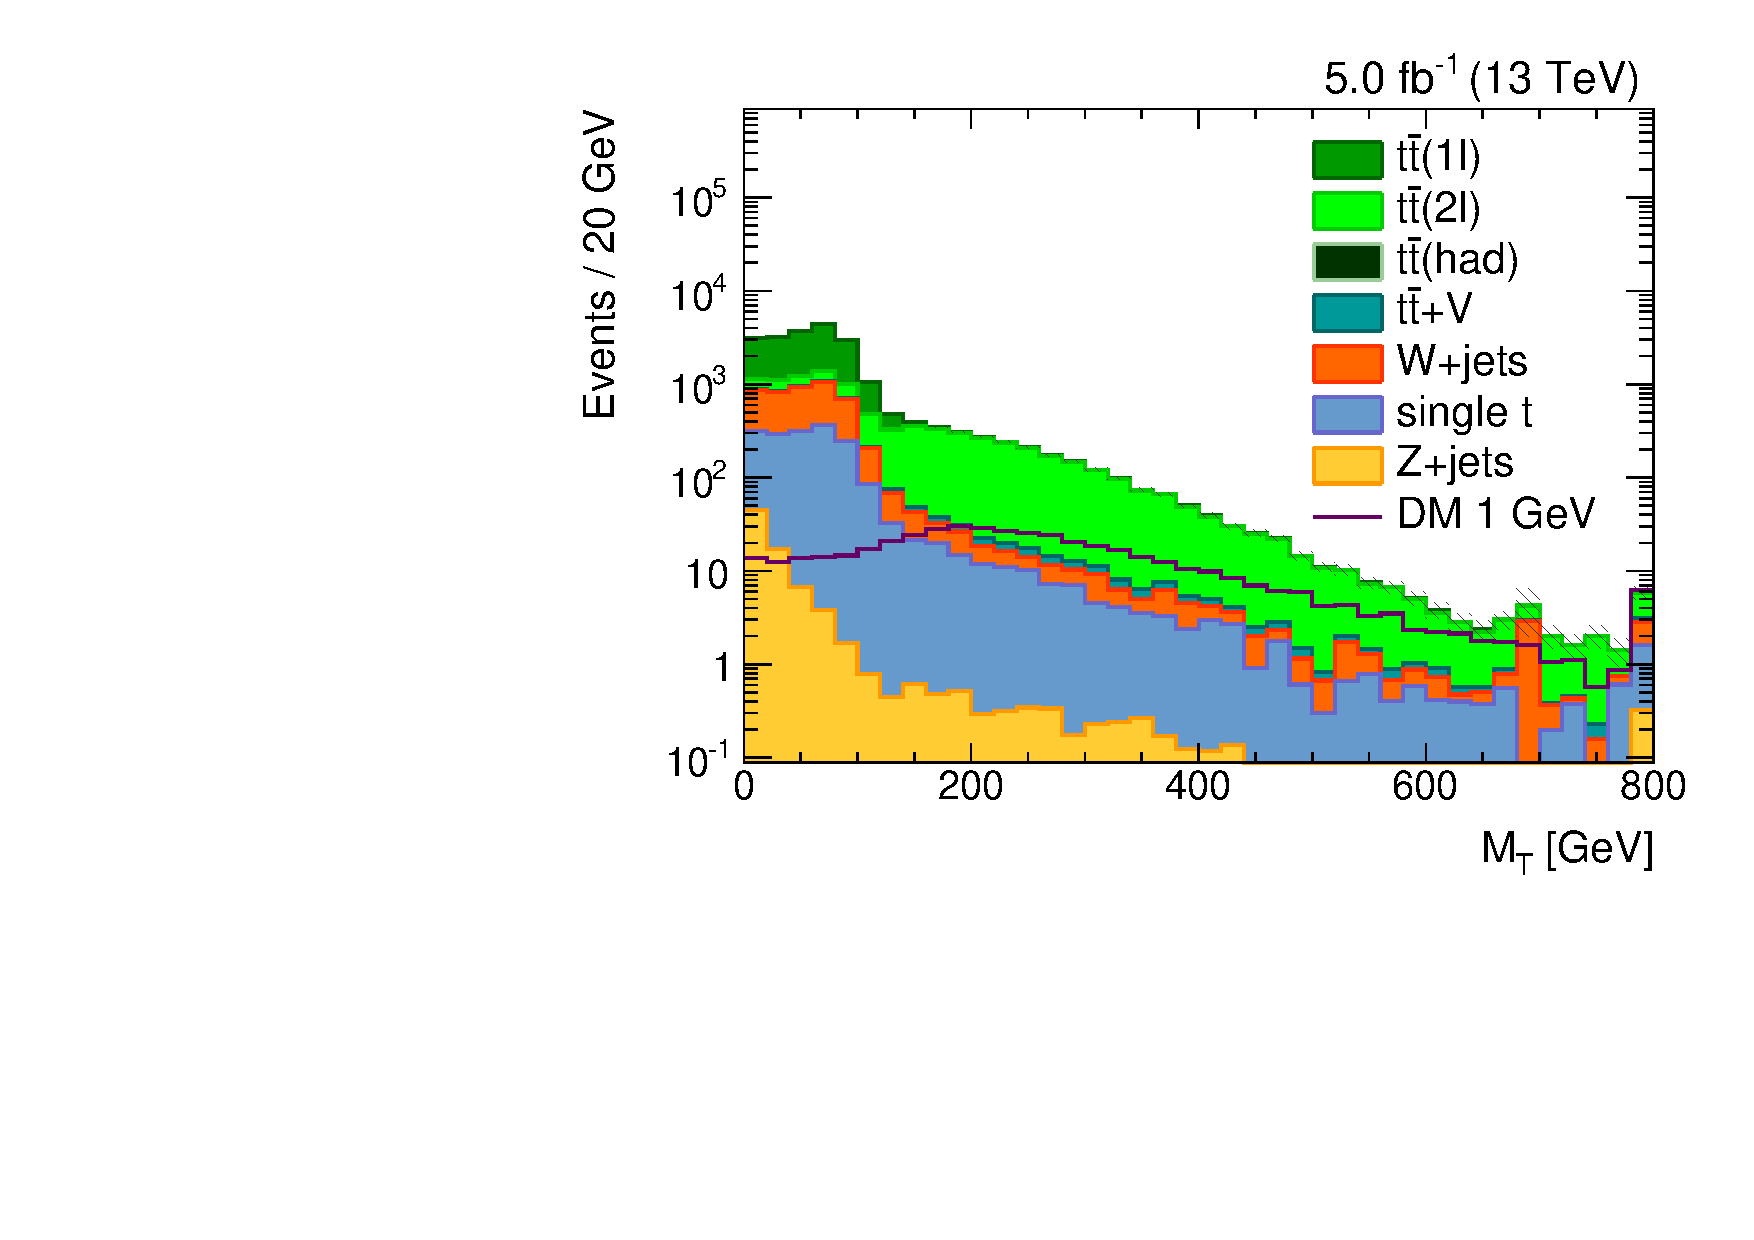
\includegraphics[width=0.48\textwidth]{figures/semilept-incl-mtlog_l.pdf}
  \caption{The $M_T$ distribution in linear (left) and log (right) scales. Note that the right-most bin includes overflow.}
  \label{fig:incl_semilept_mt}
\end{figure}

\begin{figure}[htbp]
  \centering
  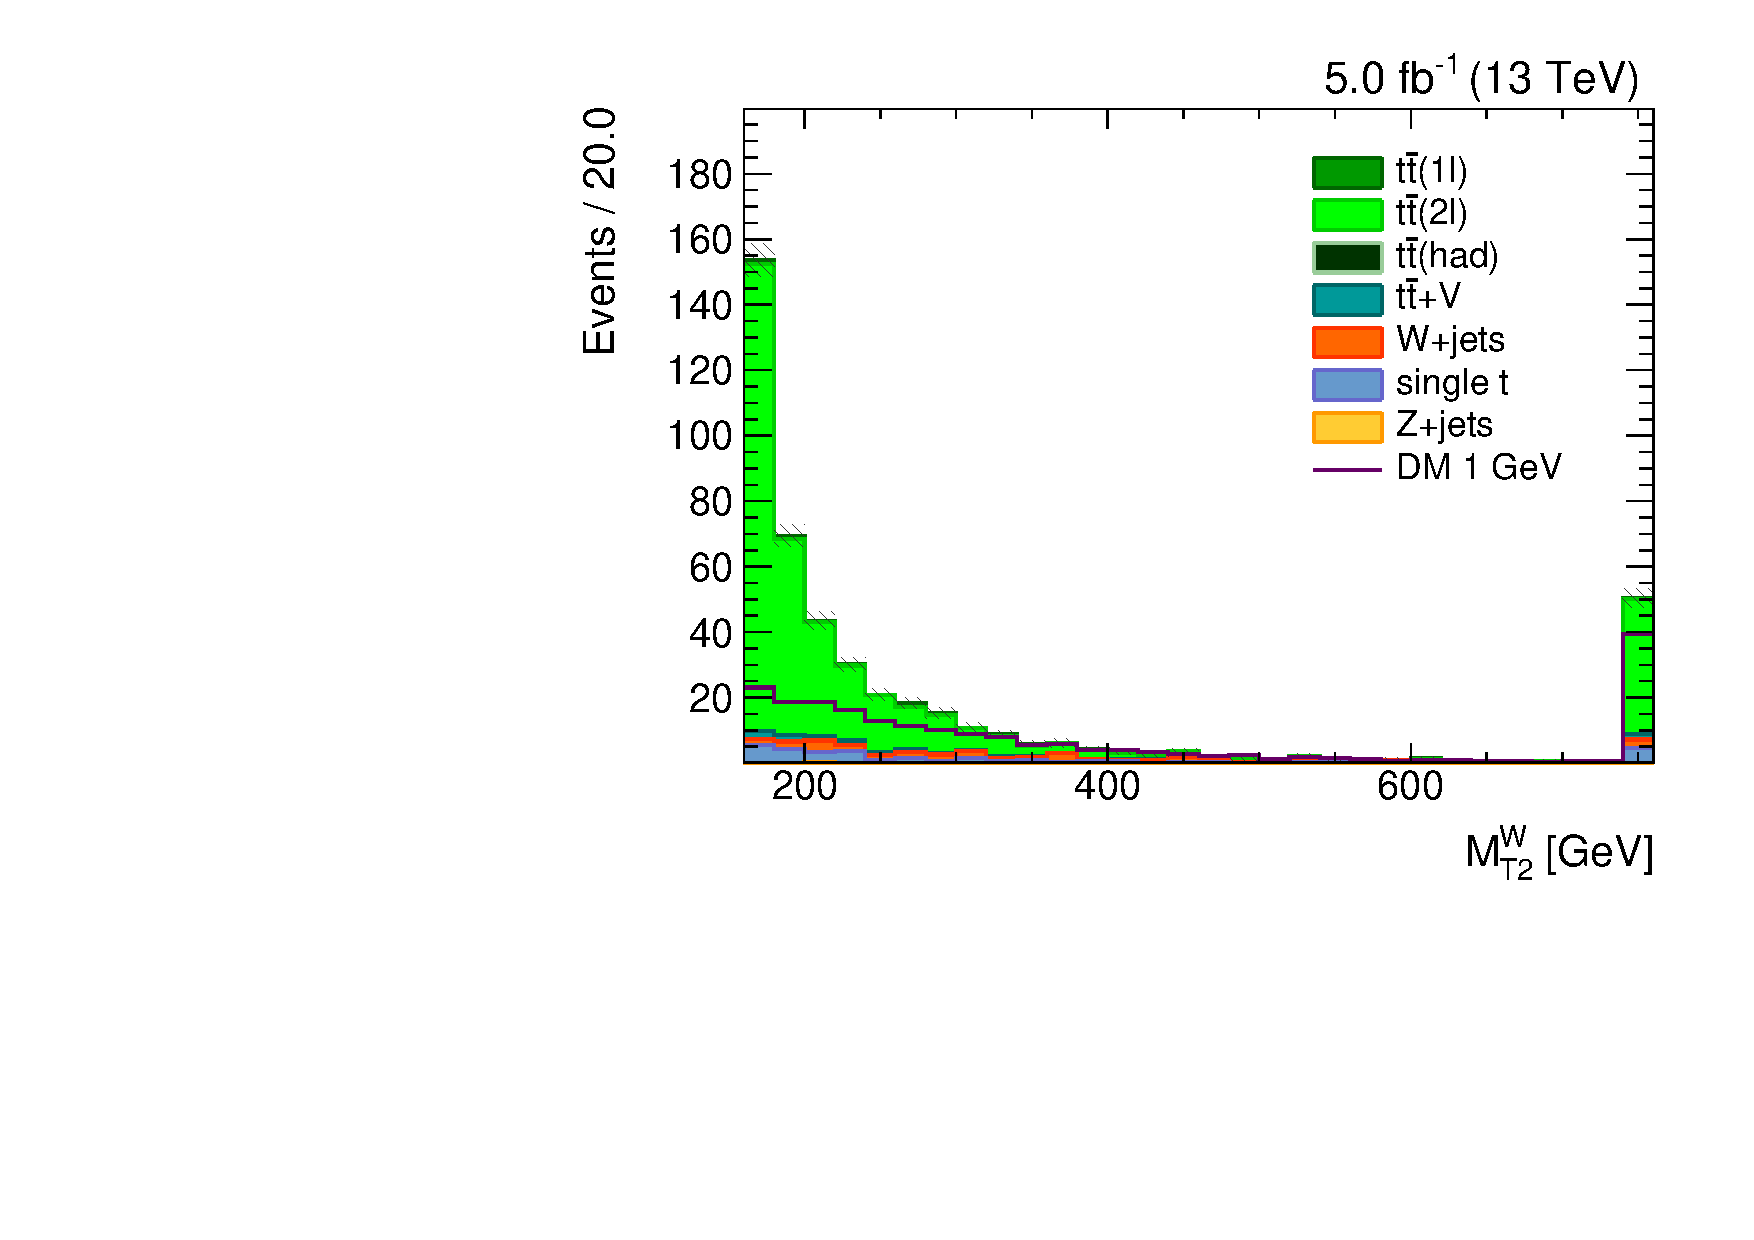
\includegraphics[width=0.48\textwidth]{figures/semilept-incl-mt2w_l.pdf}
  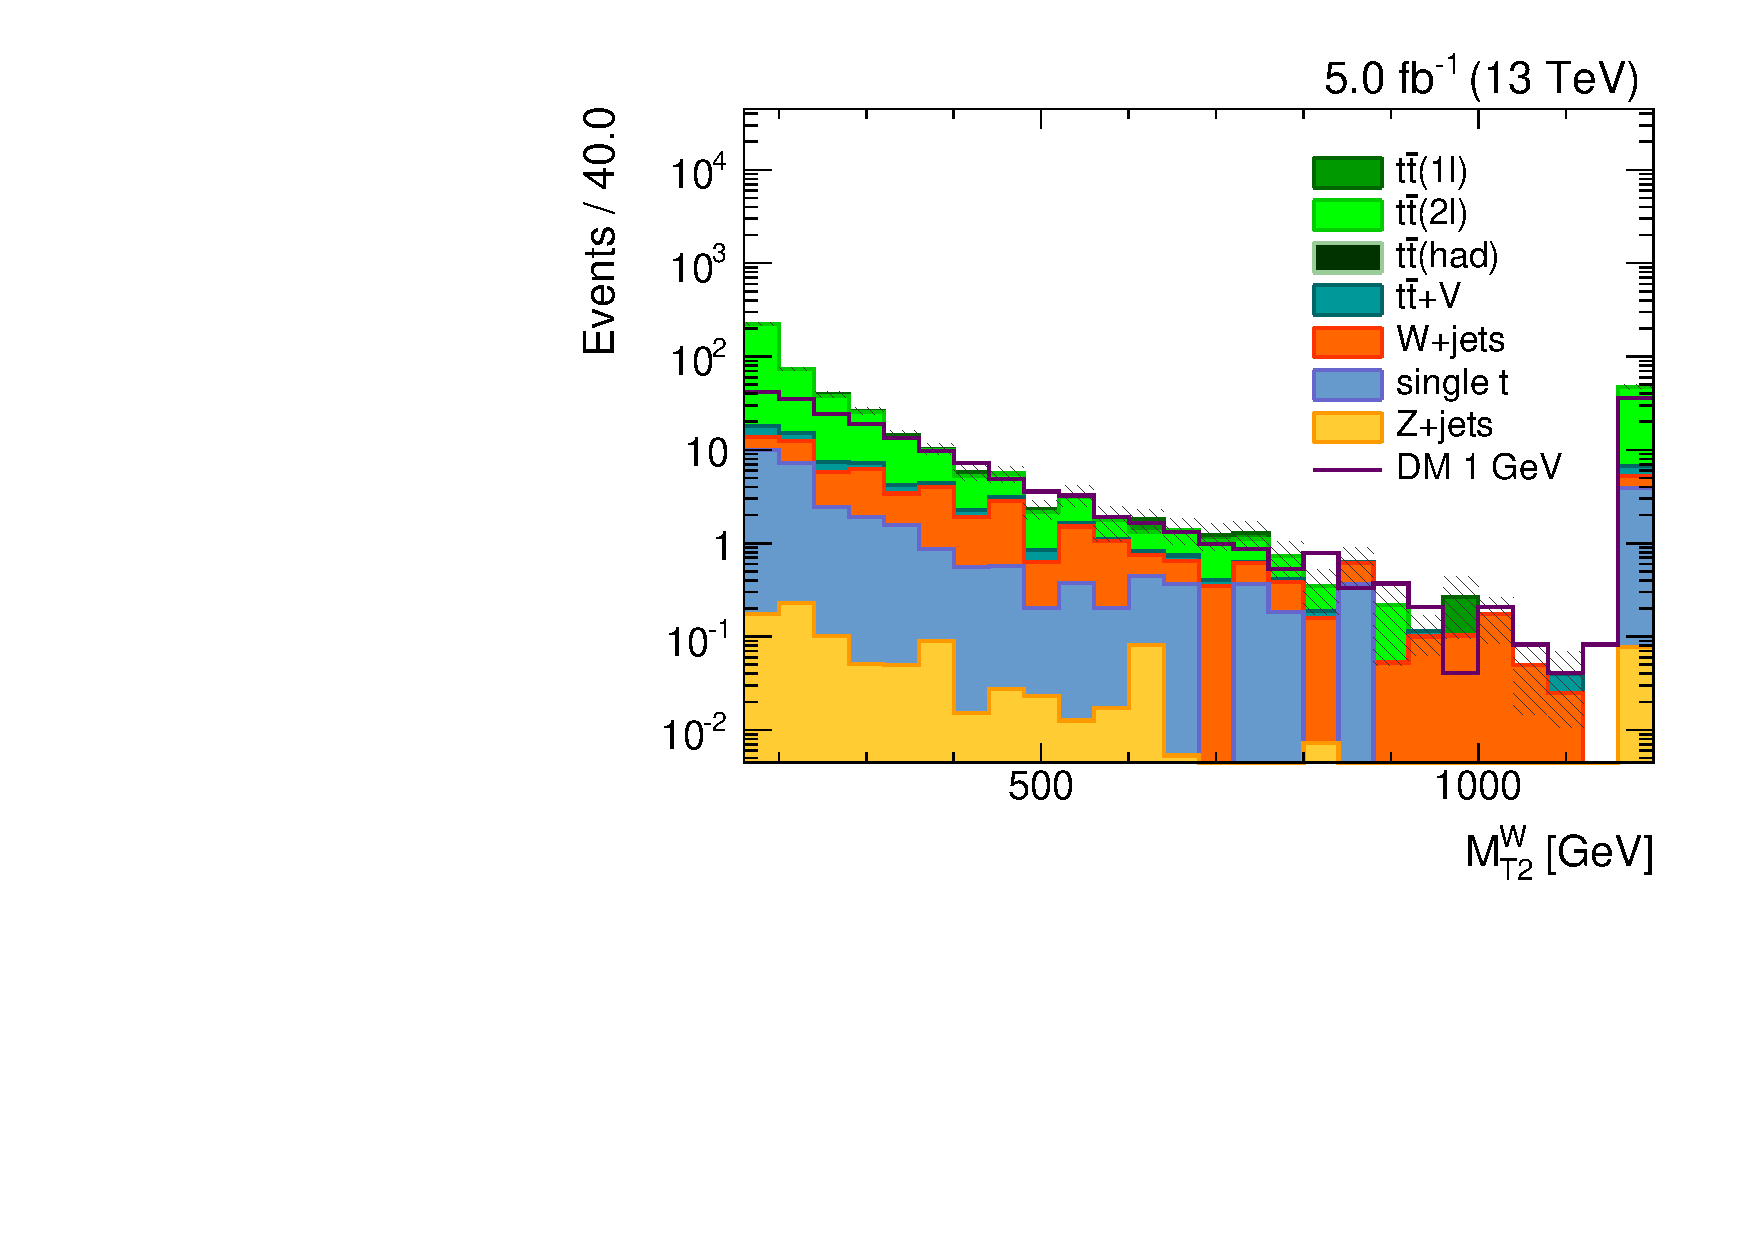
\includegraphics[width=0.48\textwidth]{figures/semilept-incl-mt2wlog_l.pdf}
  \caption{The $M_{T2}^W$ distribution in linear (left) and log (right) scales. Note that the right-most bin includes overflow.}
  \label{fig:incl_semilept_mt2w}
\end{figure}

\begin{figure}[htbp]
  \centering
  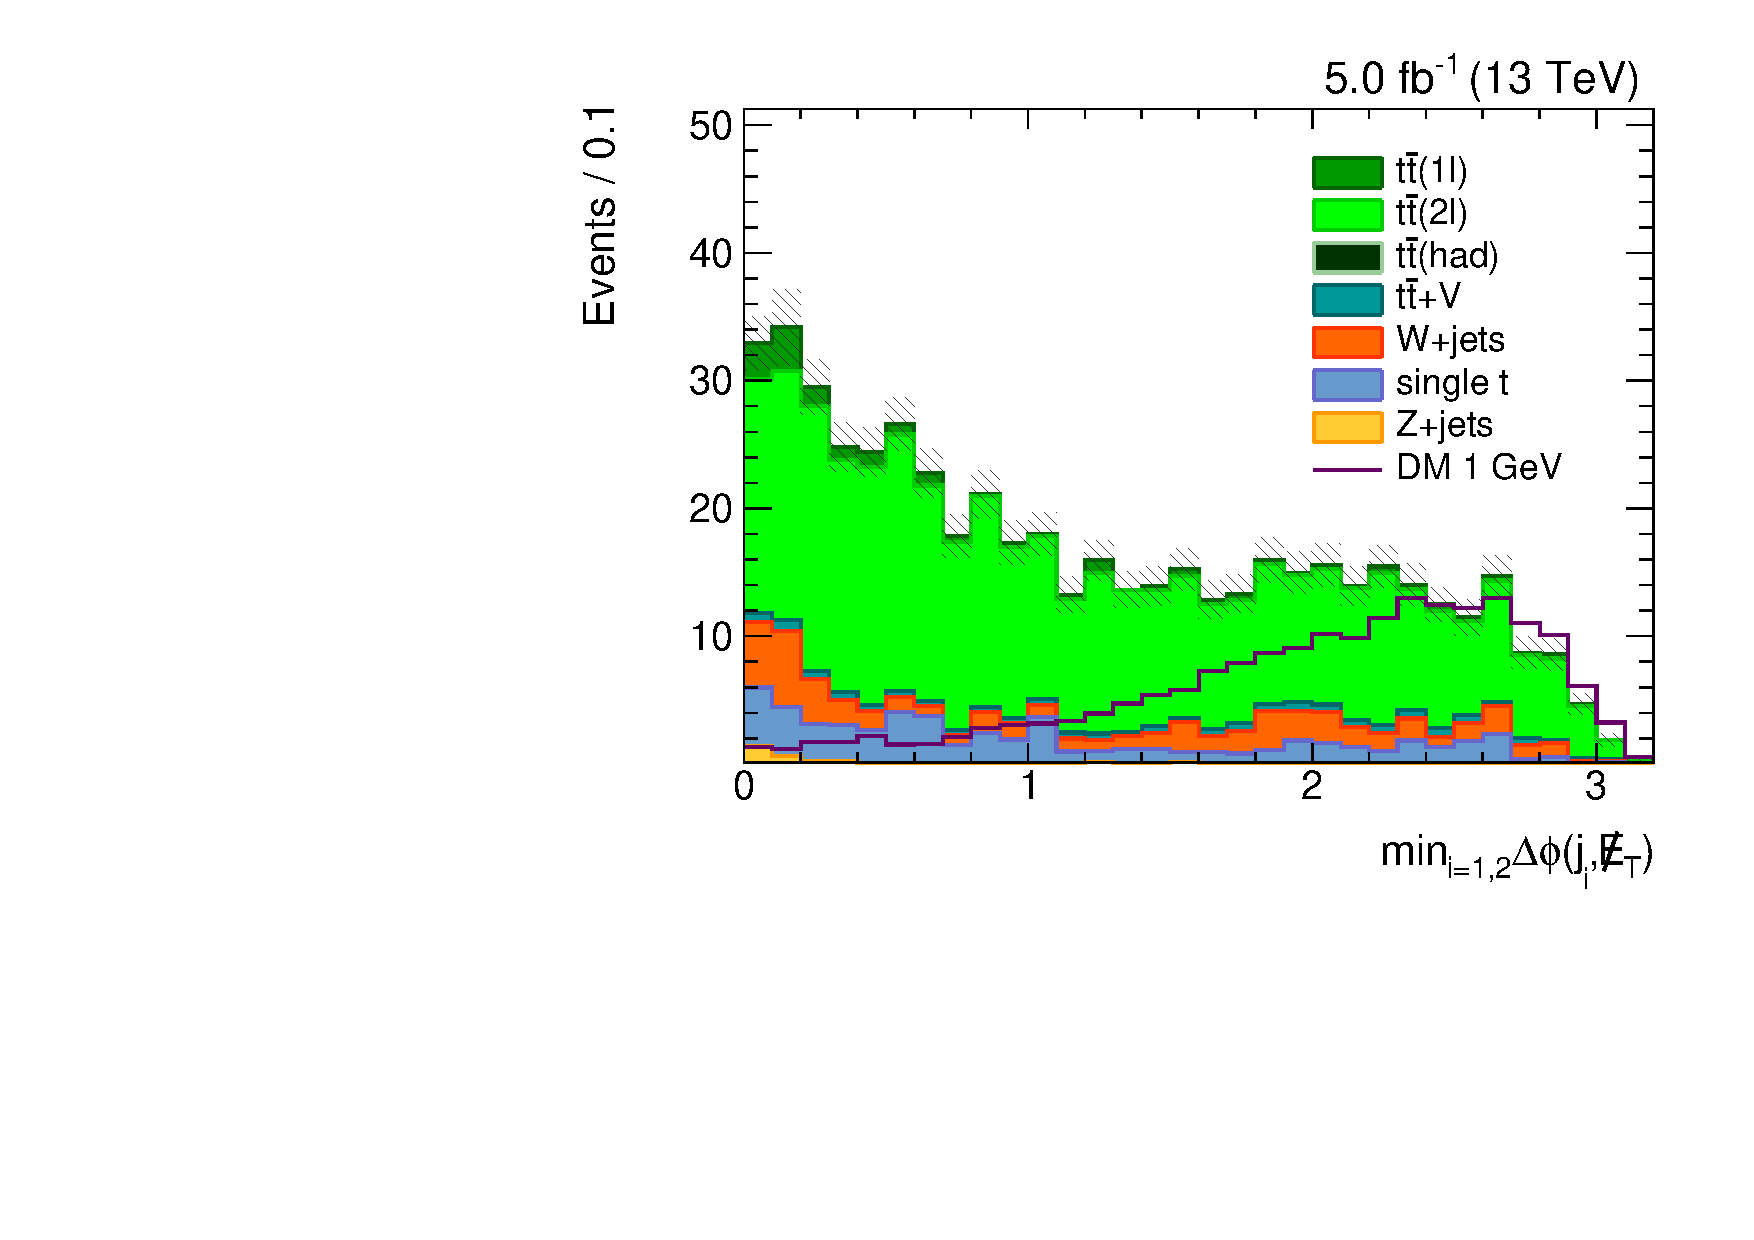
\includegraphics[width=0.48\textwidth]{figures/semilept-incl-dphijetmet2_l.pdf}
  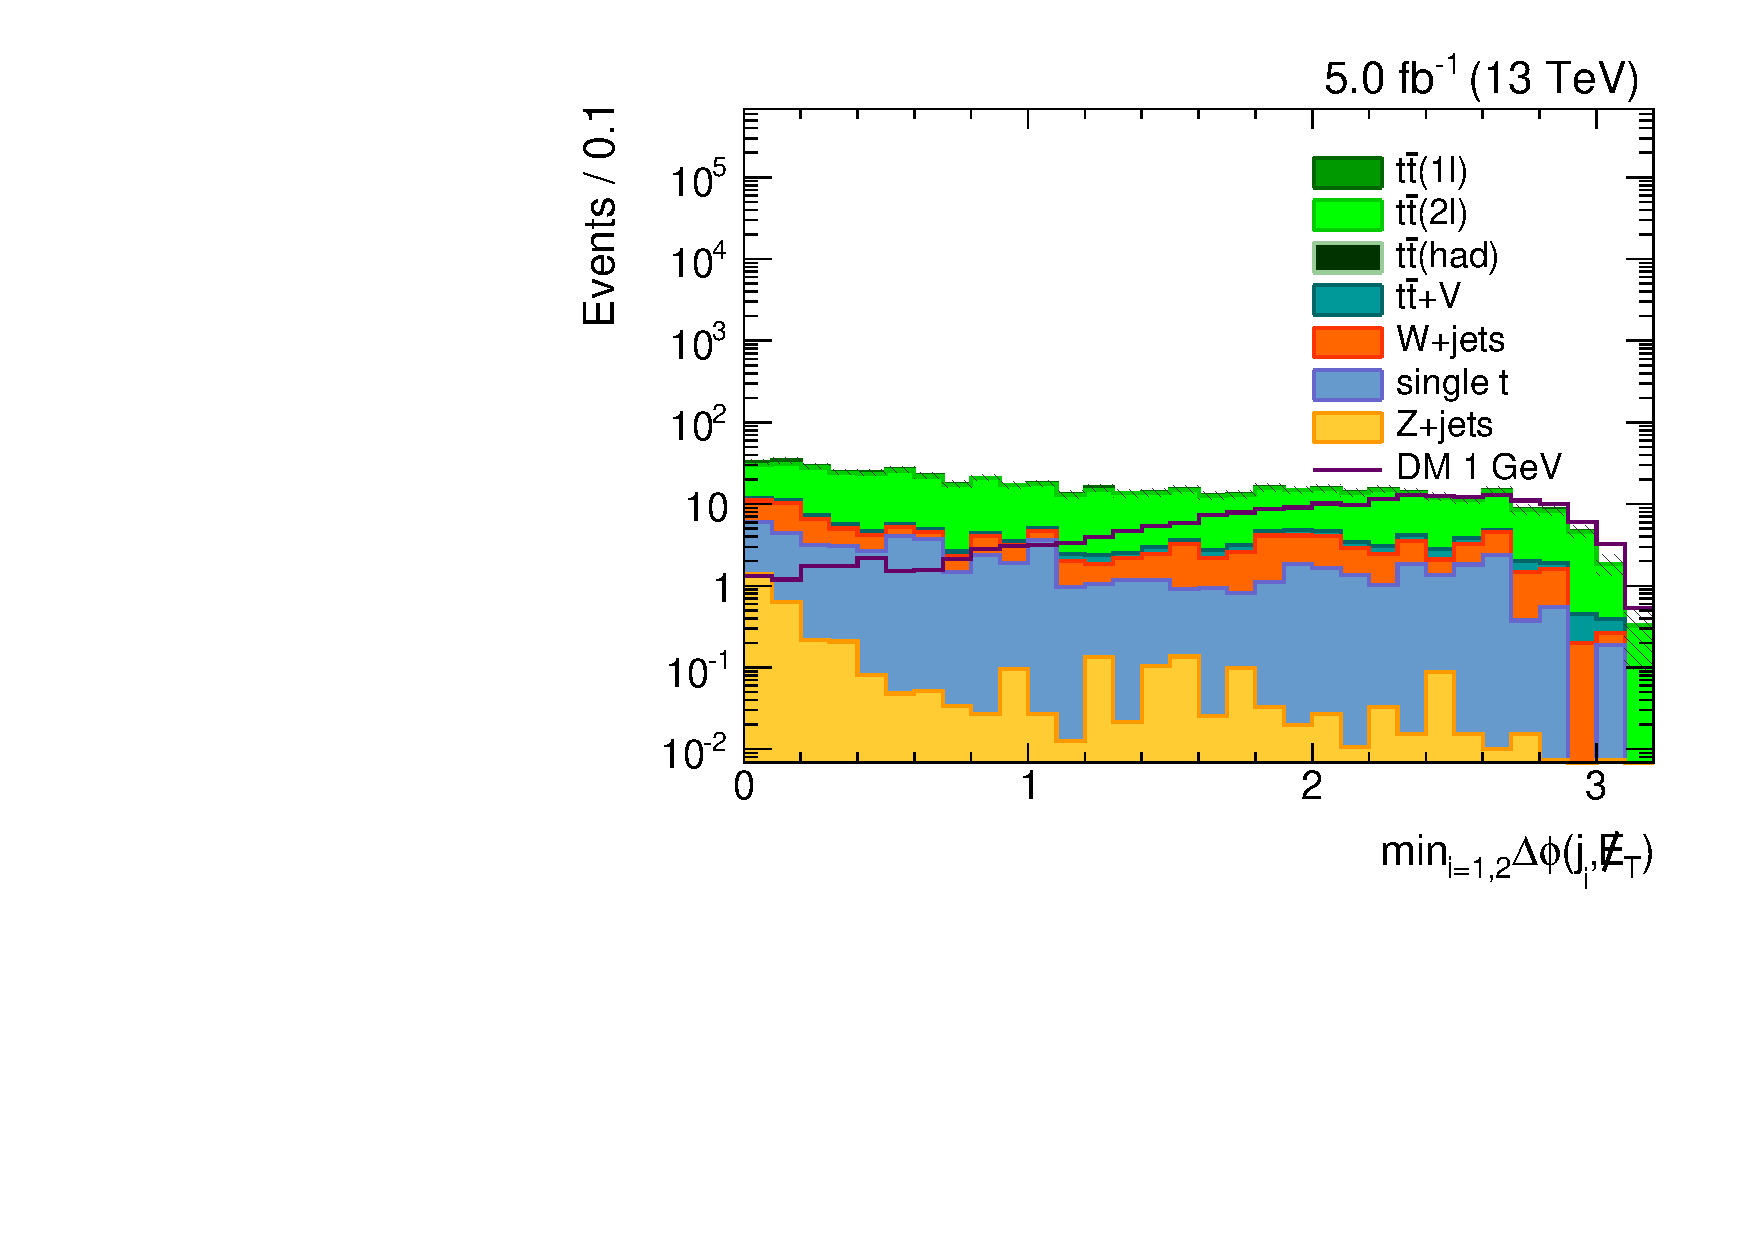
\includegraphics[width=0.48\textwidth]{figures/semilept-incl-dphijetmet2log_l.pdf}
  \caption{The $\min_{i=1,2}\Delta\phi\left(j_i\,\met\right)$ distribution in linear (left) and log (right) scales.}
  \label{fig:incl_semilept_dphijetmet2}
\end{figure}

The $\met$ distribution after selection is shown in Fig.~\ref{fig:incl_semilept_met}.
\begin{figure}[htbp]
  \centering
  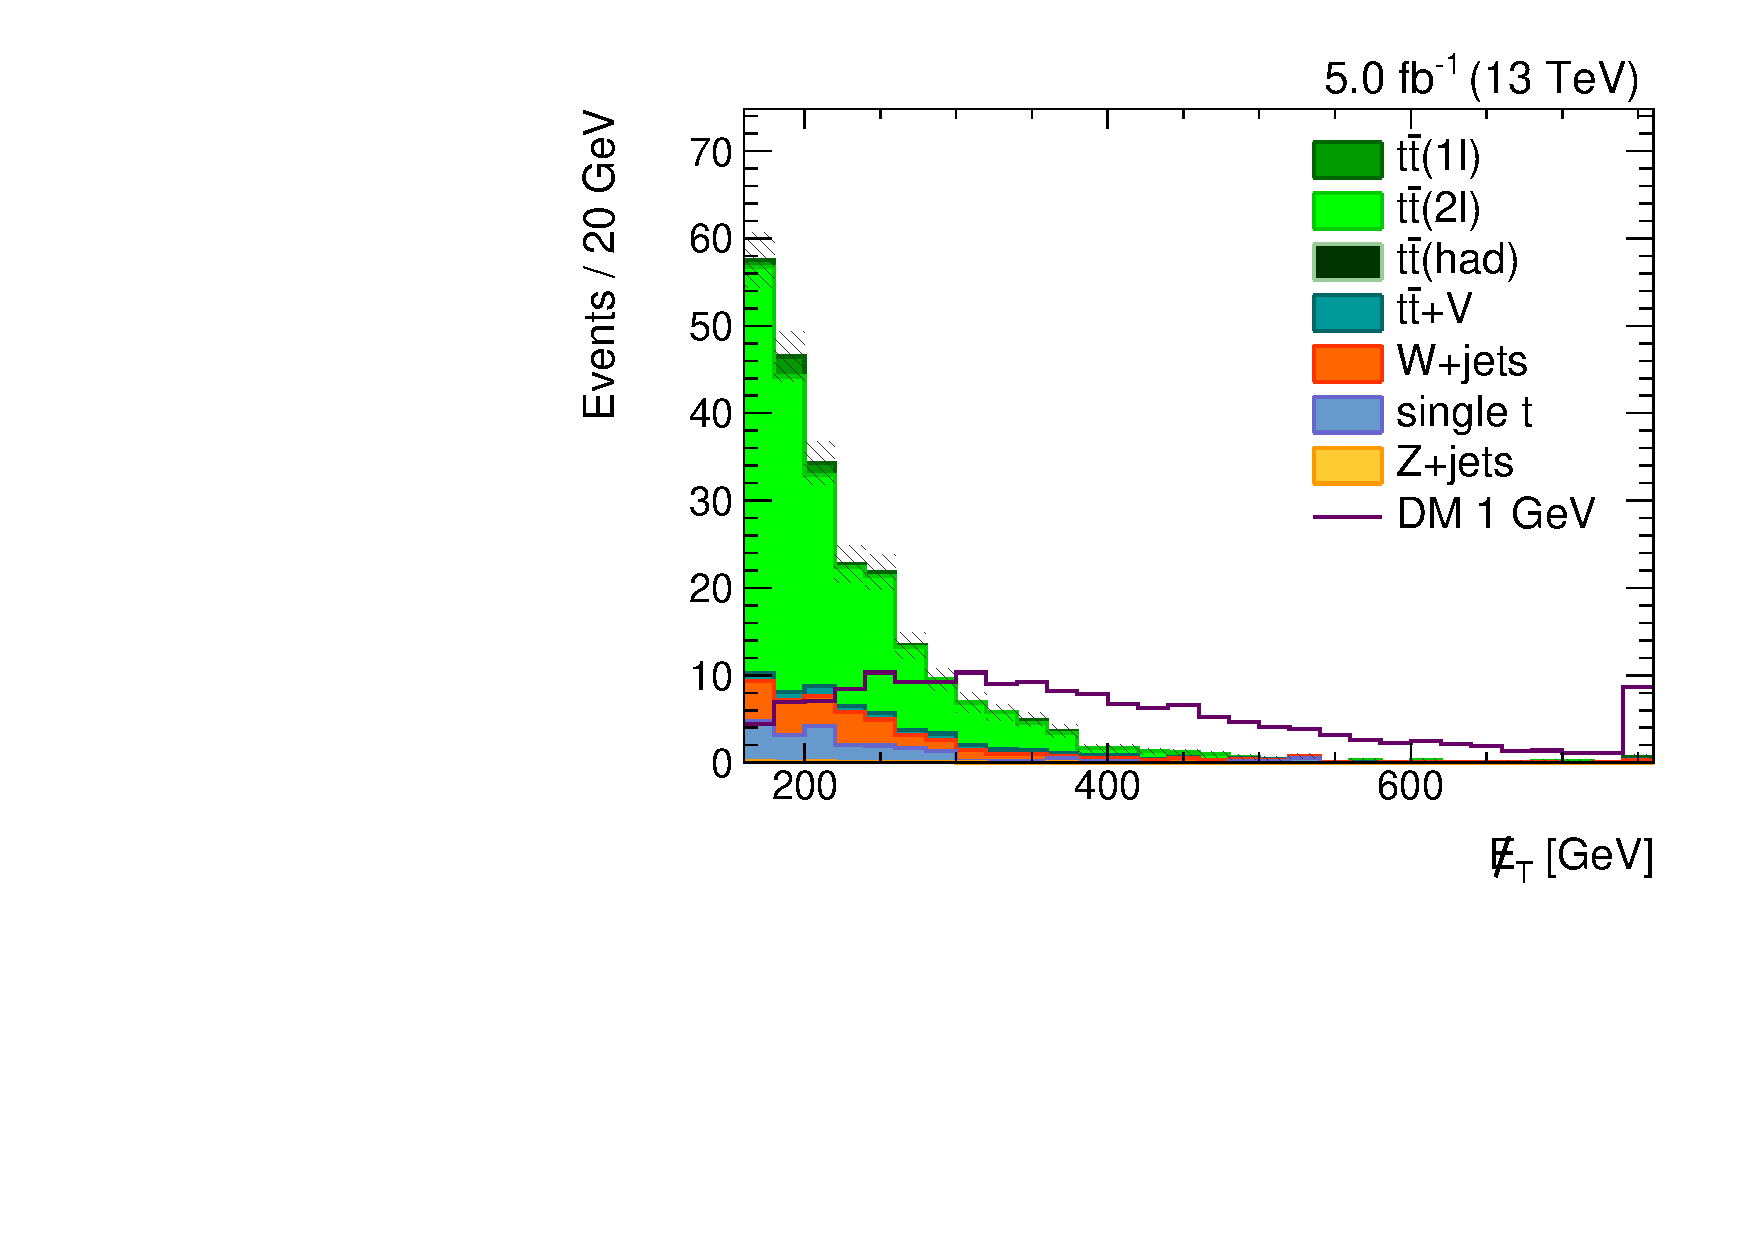
\includegraphics[width=0.48\textwidth]{figures/semilept-incl-met_l.pdf}
  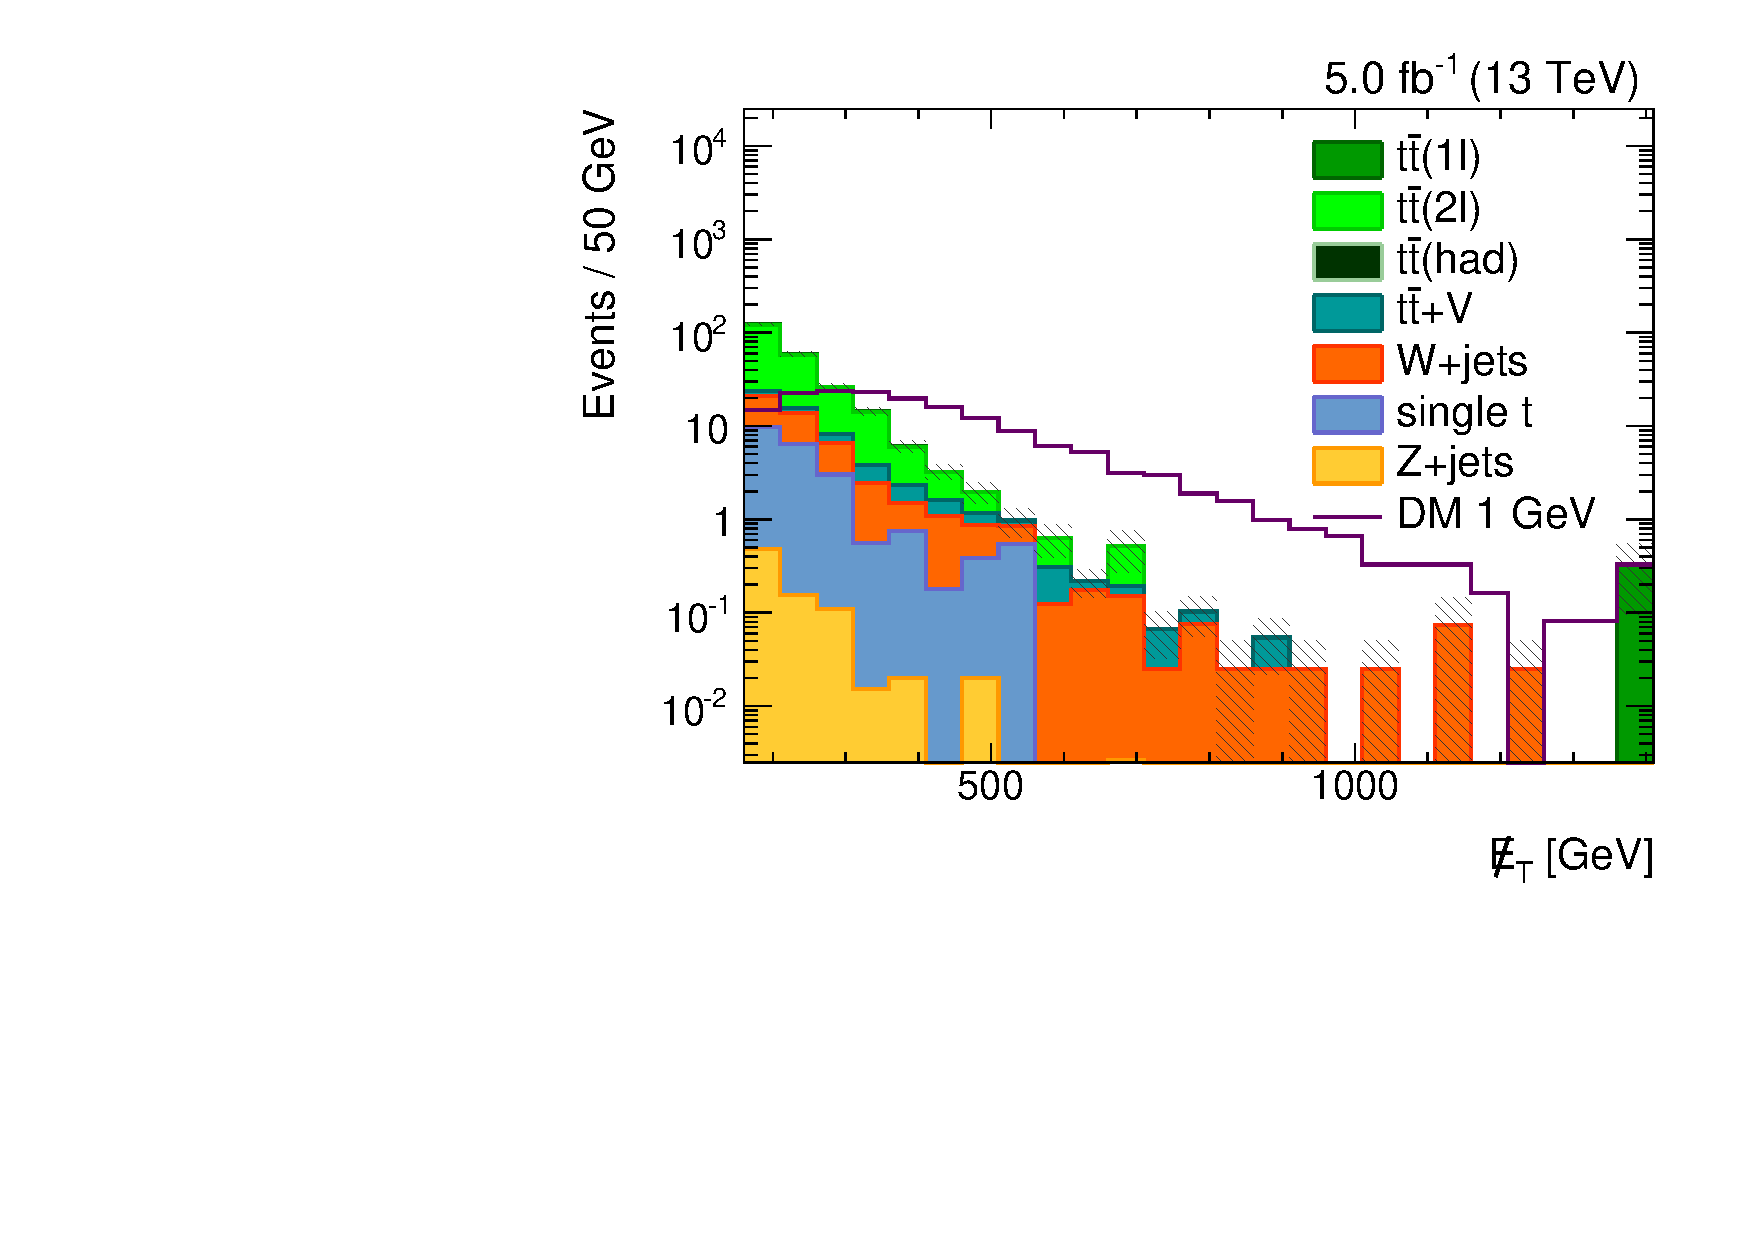
\includegraphics[width=0.48\textwidth]{figures/semilept-incl-metlog_l.pdf}
  \caption{The $\met$ distribution after semileptonic selection in linear (left) and log (right) scales. Note that the right-most bin includes overflow.}
  \label{fig:incl_semilept_met}
\end{figure}

The expected yields for $5\:\ifb$ after selection are shown in Table~\ref{tab:incl_semilept_yields}.

\begin{table}[!ht]
\centering
\begin{tabular}{|c|rr|r|}
\hline
  Process & \multicolumn{1}{|c}{$e$} & \multicolumn{1}{c|}{$\mu$} & \multicolumn{1}{|c|}{$e+\mu$} \\
\hline
  \Z\To\Lep\Lep         & $  0.28 \pm 0.09$ & $  0.52 \pm 0.14$ & $  0.80 \pm 0.17$ \\
  Single \Top           & $  7.75 \pm 1.18$ & $ 13.01 \pm 1.53$ & $ 20.76 \pm 1.93$ \\
  \Wjets                & $ 11.23 \pm 1.57$ & $ 16.31 \pm 2.35$ & $ 27.54 \pm 2.83$ \\
  $\ttbar+V$            & $  4.22 \pm 0.24$ & $  5.27 \pm 0.27$ & $  9.50 \pm 0.37$ \\
  $\ttbar\mbox{(had)}$  & $  0.00 \pm 0.00$ & $  0.00 \pm 0.00$ & $  0.00 \pm 0.00$ \\
  $\ttbar(2\Lep)$       & $ 77.30 \pm 3.55$ & $ 95.61 \pm 3.95$ & $172.91 \pm 5.32$ \\
  $\ttbar(1\Lep)$       & $  3.43 \pm 0.75$ & $  2.78 \pm 0.67$ & $  6.21 \pm 1.01$ \\

\hline
  SM expected           & $365.94 \pm 4.14$ & $133.50 \pm 4.91$ & $237.72 \pm 6.42$ \\
\hline
  $M_\chi=1\:\GeV$      & $289.61 \pm 1.75$ & $ 91.77 \pm 1.94$ & $165.93 \pm 2.61$ \\
\hline
\end{tabular}
\caption{Expected yields for $5\:\ifb$ after the inclusive selection for the semileptonic channel.}
\label{tab:incl_semilept_yields}
\end{table}
